%! suppress = Makeatletter
%! suppress = Makeatletter
\documentclass[11pt]{report}

\usepackage[T1]{fontenc}
\usepackage[utf8]{inputenc}
\usepackage{graphicx}
\usepackage{amsmath,amssymb,amsfonts}
\usepackage{polski}
\usepackage[raggedright]{titlesec}
\usepackage{indentfirst}
\usepackage{listings}
\usepackage{hyperref}
\usepackage[backend=biber, bibencoding=utf8, style=ieee, dashed=false, isbn=false, doi=false, sorting=anyvt]{biblatex}
\usepackage{caption}
\captionsetup{%
justification=raggedright,
labelfont=bf,
singlelinecheck=off
}

\addbibresource{main.bib}

\pagestyle{headings}

\renewcommand{\chaptername}{Rozdział}
\renewcommand{\contentsname}{Spis treści}
\renewcommand{\figurename}{Rys.}
\renewcommand{\tablename}{Tab.}
\renewcommand{\listfigurename}{Spis rysunków}
\renewcommand{\listtablename}{Spis tabel}
\renewcommand{\bibname}{Bibliografia}

\makeatletter
\renewcommand{\l@section}{\@dottedtocline{1}{1.5em}{2.6em}}
\renewcommand{\l@subsection}{\@dottedtocline{2}{4.0em}{3.6em}}
\renewcommand{\l@subsubsection}{\@dottedtocline{3}{7.4em}{4.5em}}
\makeatother

\begin{document}
    \begin{titlepage}
        \centering
        \center{\scshape Sieciowe Systemy Multimedialne}
        \vspace{0.05\textheight}
        \center{\textbf CYFROWE ORGANY}
        \vspace{0.06\textheight}
        \center{\LARGE\bfseries Wykorzystanie symulatora wirtualnych organów piszczałkowych w celu poprawy brzmienia istniejącego instrumentu cyfrowego}
        \center{Using a virtual pipe organ simulator to improve the sound of an existing digital instrument}
        \vspace{0.5\textheight}
        \center{Michał Patyk}
        \vspace{0.03\textheight}
        \center{Kraków 2021}
    \end{titlepage}

    \tableofcontents


    \chapter{Wstęp}\label{ch:wstęp}
    Fascynacja organami i pracą organisty towarzyszyła autorowi od lat dzieciństwa.
    Niestety elektroniczny instrument znajdujący się w parafialnym kościele wypada dość blado na tle współczesnych rozwiązań.
    Skromne możliwości finansowe parafii wciąż nie pozwalają na zakup docelowego instrumentu jakim są organy piszczałkowe których budowa to koszt rzędu kilkuset tysięcy złotych.


    \section{Motywacja}
    Motywacją do wykonania projektu jest chęć poprawy brzmienia oraz zwiększenia możliwości istniejącego instrumentu cyfrowego.


    \chapter{Przegląd dziedziny}
    W tym rozdziale opisano system MIDI~\ref{sec:midi}, organy piszczałkowe~\ref{sec:organy-piszczałkowe}, organy cyfrowe~\ref{sec:organy-cyfrowe}
    oraz wirtualne organy piszczałkowe~\ref{sec:wirtualne-organy-piszczałkowe}.


    \section{MIDI}\label{sec:midi}
    Musical Instrument Digital Interface (cyfrowy interfejs instrumentów muzycznych) to system służący do przekazywania informacji pomiędzy elektronicznymi instrumentami muzycznymi.
    Składa się z protokołu komunikacyjnego i specyfikacji sprzętowej.
    Powstał na początku lat osiemdziesiątych.
    W przeciwieństwie do strumieni audio, MIDI przekazuje cyfrową reprezentację wykonania, a nie właściwy dźwięk.

    Jak podaje~\cite{122929520160101}, są trzy typy portów MIDI: IN, OUT i THRU.
    Serializowane dane przesyłane są w kablu w jednym kierunku.
    MIDI OUT to wyjście danych do innego urządzenia.
    MIDI IN to wejście danych z innego urządzenia.
    MIDI THRU przekazuje wszystkie wiadomości które dotrą do urządzenia na port MIDI IN.

    Wiadomości MIDI sa podzielone na dwie kategorie: wiadomości systemowe i wiadomości kanałów.
    Wiadomości systemowe to te które sa związane z całym systemem MIDI.
    W każdej wiadomości kanałowej może być zakodowane do 16 kanałów, co pozwala na przesłanie jednym kablem wykonania składającego się z 16 różnych źródeł dźwięku.


    \section{Organy piszczałkowe}\label{sec:organy-piszczałkowe}
    Organy piszczałkowe~\cite{329316420170801}, to jeden z najstarszych, wciąż często wykorzystywanych, instrumentów.
    Jednocześnie jest to największy i najbardziej złożony instrument.
    Najprostsze organy składają się z pojedynczego zestawu piszczałek, klawiatury (zwanej manuałem) w której każdy klawisz uwalnia powietrze do odpowiedniej piszczałki oraz urządzenia wytwarzającego ciśnienie powietrza.
    Bardziej złożone organy mają wiele rejestrów (zestawów piszczałek), kilka manuałów oraz pedał (klawiaturę nożną).
    Piszczałki mogą być skonstruowane z metalu lub drewna.
    Ich długość zaczyna się od kilku centymetrów, a może dochodzić do nawet 32 stóp (prawie 10 metrów).


    \section{Organy cyfrowe}\label{sec:organy-cyfrowe}
    Organy cyfrowe posiadają rozmaitą paletę głosów.
    Odwzorowanie brzmienia organów piszczałkowych tworzone jest najczęściej poprzez syntezę addytywną.
    W takim rodzaju syntezy przebiegi fal dźwiękowych nie są zapisywane bezpośrednio.
    Zamiast tego przechowywane są listy liczb określające amplitudy każdej harmonicznej,
    które są następnie wykorzystywane do tworzenia dźwięków w czasie rzeczywistym, zgodnie z wymaganiami.
    Kontuar (stół gry) organów cyfrowych zwykle wyglądem bardzo przypomina ten z organów piszczałkowych.
    Zgodnie z instrukcją Konferencji Episkopatu Polski organy elektroniczne wolno stosować tylko jako instrument tymczasowy,
    bez dodawania sztucznego prospektu (frontowej elewacji zewnętrznej).


    \section{Wirtualne organy piszczałkowe}\label{sec:wirtualne-organy-piszczałkowe}

    \begin{figure}[!ht]
        \centering
        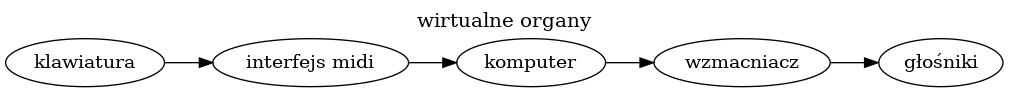
\includegraphics[width=\linewidth]{fig/organizacja.png}
        \caption{Schemat wykorzystania wirtualnych organów. (źródło:~opracowanie własne)}
        \label{fig:schemat}
    \end{figure}

    Komputer z odpowiednim oprogramowaniem może stać się symulatorem organów piszczałkowych.
    Dzięki wykorzystaniu próbek dokładnie odtwarza on brzmienie każdej piszczałki.
    Słyszalne są wszystkie szumy, stuki mechanizmu, do tego stopnia, że jest wręcz nie do odróżnienia, czy to grają wirtualne organy, czy też historyczny instrument.
    Próbki dźwięków zarejestrowane za pomocą mikrofonów zostają przypisane konkretnym klawiszom i pedałom.
    Rysunek~\ref{fig:schemat} przedstawia schemat wykorzystania typowych wirtualnych organów.

    \subsection{Sampling}
    Sampling to technika nagrywania dźwięków instrumentu muzycznego.
    Najprostsze rozwiązania to takie w których nagrywa się tylko kilka dźwięków, podczas gdy pozostałe są tworzone przez transponowanie.
    Najlepsze zestawy próbek to te w których każdy dźwięk jest nagrywany osobno.
    Niestety takie rozwiązanie, poza pracochłonnością procesu nagrywania, niesie też ze sobą problemy natury technicznej.
    Dźwięki powinny być przechowywane w najlepszym możliwie formacie, przy jak najwyższej częstotliwości próbkowania oraz wielobitowej kwantyzacji.
    W rezultacie powstaje duża ilość danych (kilka - kilkanaście gigabajtów).
    Dla najlepszej wierności dźwięku stosuje się tak zwane próbkowanie multi-release,
    w którym dla każdej piszczałki nagrywa się próbki rozpoczęcia, podtrzymania oraz wiele próbek zanikanie dźwięku.
    Taki zabieg wynika z faktu, że dźwięk zanikania ma inny charakter w zależności od długości nuty.
    Związane jest to z akustyką kościołów i hal koncertowych.
    Poza dźwiękami piszczałek, dla dodania realizmu, dołącza się też dźwięki mechanizmów, a nawet dmuchaw.

    \subsection{Oprogramowanie}

    Na rynku wirtualnych organów piszczałkowych istnieją dwaj duzi gracze: Hauptwerk oraz GrandOrgue.

    \paragraph{Hauptwerk}
    Hauptwerk to komercyjny program komputerowy stworzony w 2002 roku przez Martina Dyde'a~\cite{13115512220180101}, wydawany przez Milan Digital Audio.
    Występuje w wielu wersjach.
    Jest dostępny jako comiesięczna subskrypcja lub licencja.
    Ceny wahają sie od 12.99\$ miesięcznie do 599\$ za wieczystą licencję~\cite{hauptwerk}.
    Program umożliwia tworzenie muzyki organowej przy wykorzystaniu MIDI i próbek dźwiękowych.

    \paragraph{GrandOrgue}
    GrandOrgue to darmowe oprogramowanie o otwartym kodzie źródłowym~\cite{grandorgue}.
    Jest rozwijany przez społeczność od 2009 roku w serwisie Sourceforge.
    Oferuje teraz funkcje i realizm zbliżony do Hauptwerk.
    Aktualizacje są bezpłatne.
    Użycie zwykłych zestawów próbek wave i udokumentowanego formatu ODF zapewni kompatybilność w przyszłości.


    \chapter{Koncepcja}
    W tym rozdziale opisany został stan istniejący~\ref{sec:stan-istniejący} oraz cele realizacji projektu~\ref{sec:cele}.


    \section{Stan istniejący}\label{sec:stan-istniejący}

    \begin{figure}[!ht]
        \centering
        \includegraphics[width=\linewidth]{fig/organyViscount.jpg}
        \caption{Organy Viscount Classic 4500. (źródło:~opracowanie własne)}
        \label{fig:organyViscount}
    \end{figure}

    Cyfrowe organy Classic 4500 firmy Viscount~\ref{fig:organyViscount}.
    Posiadają dwa manuały po 56 klawiszy i 27 klawiszowy pedał.
    Generacja dźwięku przebiega na zasadzie syntezy addytywnej.
    Organy posiadają wyjście i wejście midi w postaci dwóch 5 pinowych złączy DIN.
    Wyjście dźwiękowe organów jest podłączone do mikser.

    Mikser XRD 680S firmy Peavey z wbudowanymi efektami i wzmacniaczem o mocy 150W na kanał.
    Posiada frontowy panel z wyjściami i monitorem poziomu, a także kontrole wysokich, średnich i niskich tonów.


    \section{Cele}\label{sec:cele}
    Głównym celem projektu jest poprawa brzmienia instrumentu poprzez zastąpienie dźwięku syntezowanego addytywnie,
    w istniejącym instrumencie, systemem komputerowym z wirtualnymi organami.
    Dodatkowym celem jest poszerzenie gamy dostępnych barw głosowych organów.

    Szczególnym ograniczeniem projektu jest minimalizacja kosztów wykonania.
    Wskazane jest skupienie na wykorzystaniu istniejącego sprzętu.


    \chapter{Realizacja}


    \section{Wybór sprzętu i oprogramowania}
    W celu minimalizacji kosztów zdecydowano się wykorzystać dostępny komputer.
    Przy wyborze oprogramowania ponownie kierowano się kosztem - wybór padł na darmowe oprogramowanie GrandOrgue.


    \section{Przygotowanie wirtualnych organów}

    \subsection{Instalacja systemu operacyjnego Linux}
    Jako system operacyjny wykorzystano darmowy Linux Mint~\cite{mint}.
    Proces instalacji jest łatwy i przyjazny dla użytkownika.

    \subsection{Instalacja oprogramowania GrandOrgue}
    Aby zainstalować GrandOrgue na systemie operacyjnym Linux Mint należy dodać repozytorium ze strony~\cite{grandorgueRepo},
    a następnie użyć poleceń systemowych do instalacji.
    \begin{verbatim}
        sudo apt update
        sudo apt install grandorgue
    \end{verbatim}

    \subsection{Wybór i pobranie próbek}
    Oprogramowanie GrandOrgue jest domyślnie wyposażone w podstawowy zestaw dźwięków.
    Zdecydowano się na zmianę próbek na takie o wyższej jakości.
    Należy je dołączyć do systemu ręcznie.
    W internecie dostępnych jest bardzo wiele amatorsko oraz profesjonalnie opracowanych próbek.
    Zdecydowano się wykorzystać darmowe sample udostępniane przez stronę Piotra Grabowskiego~\cite{grabowski}.
    Przygotowane przez autora zestawy są wysokiej jakości.
    Mają dobrze zaprojektowane i atrakcyjne interfejsy użytkownika.
    W niczym nie ustępują zestawom komercyjnym.

    Spośród dostępnych instrumentów wybrano dwa posiadające dwa manuały oraz pedał (dla zgodności z istniejącymi organami elektronicznymi):
    \begin{enumerate}
        \item mniejszy - Azzio - 11 rejestrów,
        \begin{enumerate}
            \item 24 bit - 4.6 GB
            \item 16 bit - 2.3 GB
        \end{enumerate}
        \item większy - Długa Kościelna - 22 rejestry.
        \begin{enumerate}
            \item 24 bit - 11.1GB
            \item 16 bit - 2.7 GB
        \end{enumerate}
    \end{enumerate}
    Powyżej, przy rozdzielczościach bitowych próbek, podano zapotrzebowanie na wolną pamięć RAM w systemie.
    Wszystkie dźwięki są przygotowane z częstotliwością próbkowania 48 kHz.

    \subsection{Podłączenie elementów zestawu}
    Przygotowany system komputerowy został podłączony do istniejących organów przy pomocy konwertera MIDI-USB pokazanego na rysunku~\ref{fig:midiusb}.
    Należy zwrócić uwagę na odpowiednią konfigurację - MIDI IN urządzenia łączymy z MIDI OUT wtyczki.
    Konwerter nie wymaga instalacji dodatkowych sterowników.
    Jest rozpoznawany przez system zaraz po podłączeniu.

    \begin{figure}[!htp]
        \centering
        \includegraphics[width=\linewidth]{fig/midi-usb.jpg}
        \caption{Konwerter MIDI-USB. (źródło:~opracowanie własne)}
        \label{fig:midiusb}
    \end{figure}

    Dźwięk generowany przez wirtualne organy jest przesyłany kablem jack - RCA (chinch) do wzmacniacza.
    Wzmacniacz zasila cztery kolumny pasywne rozmieszczone symetrycznie po dwóch stronach kościoła.

    \subsection{Konfiguracja oprogramowania}

    \paragraph{Dźwięk}
    Błędna konfiguracja programu GrandOrgue może prowadzić do silnych zniekształceń generowanego dźwięku, a w konsekwencji nawet do uszkodzenia głośników i wzmacniacza.
    Z jednej strony przyczyną zniekształceń jest wybranie zbyt niskiej jakości.
    Z drugiej strony wybranie zbyt wysokiej jakości dźwięku może spowodować niezmieszczenie się próbek w pamięci RAM.
    W takim przypadku dane mogą nie zostać dostarczone do bufora dźwięku na czas, co będzie przyczyną głośnych trzasków.

    Rysunek~\ref{fig:ustawienia-dzwieku} przedstawia ustawienia dźwięku programu GrandOrgue.
    \begin{figure}[!ht]
        \centering
        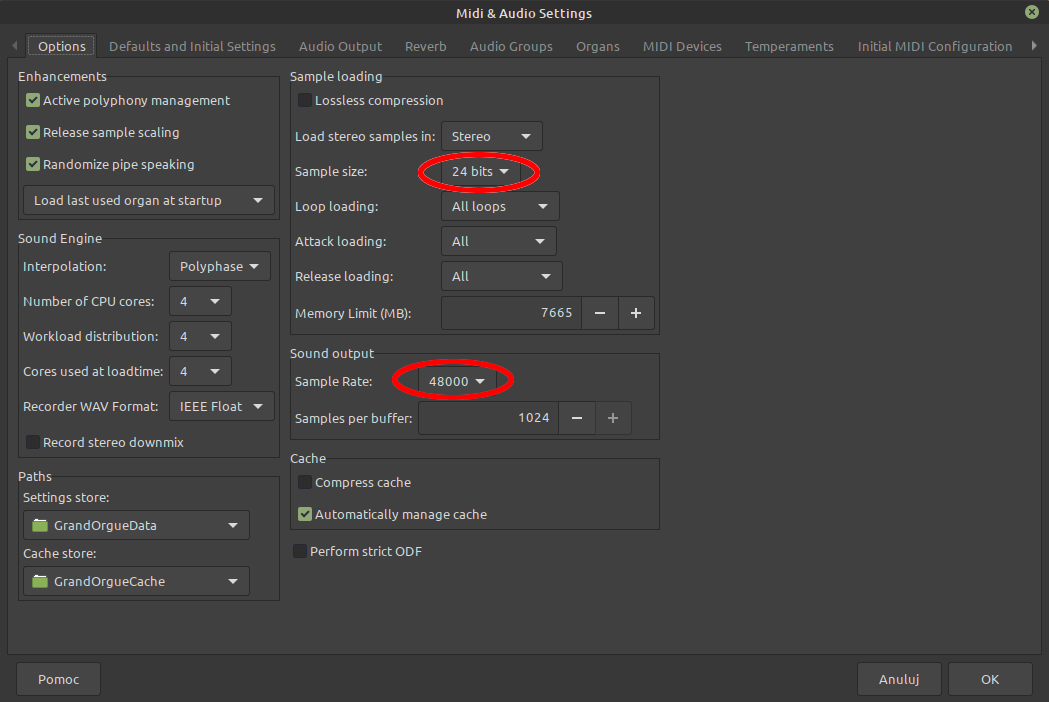
\includegraphics[width=\linewidth]{fig/optionsR.png}
        \caption{Panel ustawień dźwięku programu GrandOrgue. (źródło:~opracowanie własne)}
        \label{fig:ustawienia-dzwieku}
    \end{figure}

    Należy upewnić się, że rozdzielczość bitowa jest ustawiona zgodnie z załadowanym zestawem.
    Ustawienie innej wartości może powodować resampling w warstwach stosu audio, na czym ucierpi jakość.
    Mniejsza wartość jest dopuszczalna ale znacząco wpłynie na jakość dźwięku który stanie się wyraźnie ``płaski''.

    Ustawiony limit pamięci powinien być zgodny z ilością pamięci RAM dostępnej w systemie.

    Częstotliwość próbkowania dźwięku jest kolejną kluczową wartością dla jakości generowanego sygnału.
    Podobnie jak dla rozdzielczości bitowej, także w tym przypadku ustawienie innej wartości niż ta z zestawu może skutkować resamplingiem i pogorszeniem jakości.

    Należ też zwrócić uwagę na poziom głośności w programie, tak aby uniknąć przycinania.

    Ważną grupą ustawień są też parametry samych organów, które można zobaczyć na rysunku~\ref{fig:organy}.
    W panelu tym można dostosować głośność poszczególnych rejestrów, a także zobaczyć jaką ilość pamięci RAM zajmują.
    Możliwa jest też zmiana jakości lub wyłączenie ładowania poszczególnych sampli dla zaoszczędzenia pamięci.
    \begin{figure}[!ht]
        \centering
        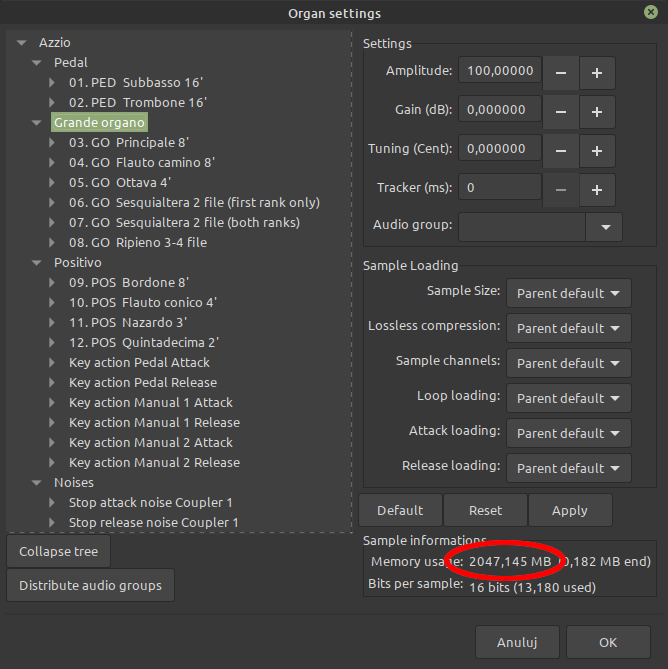
\includegraphics[width=\linewidth]{fig/organR.png}
        \caption{Panel ustawień organów. (źródło:~opracowanie własne)}
        \label{fig:organy}
    \end{figure}

    \paragraph{MIDI}
    W celu skorzystania z wirtualnych organów przy pomocy klawiatur z organów elektronicznych,
    należy wskazać programowi GrandOrgue które wiadomości MIDI odpowiadają któremu manuałowi.
    Aby to zrobić wystarczy kliknąć prawym przyciskiem myszy na wybrany manuał w programie.
    W oknie które sie pojawi należy wybrać ``Listen for event'', a następnie nacisnąć klawisz na odpowiednim manuale.
    \begin{figure}[!ht]
        \centering
        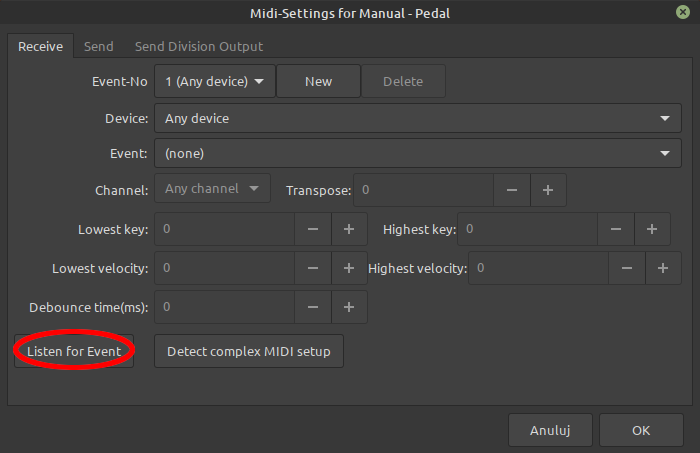
\includegraphics[width=\linewidth]{fig/midiR.png}
        \caption{Panel konfiguracji MIDI dla manuału. (źródło:~opracowanie własne)}
        \label{fig:midi}
    \end{figure}

    \paragraph{Equalizer}
    W calu uwydatnienia wybranych częstotliwości możemy dodatkowo wykorzystać programowy korektor dźwięku.
    Należy jednak pamiętać, że dodatkowe programowe przetwarzanie w torze dźwiękowym wiąże się z niepożądanym opóźnieniem (nawet kilkuset milisekund).


    \chapter{Ewaluacja}
    W tym rozdziale przeprowadzono ewaluacje podzieloną na dwie części: ocenę wrażeń słuchowych~\ref{sec:wrażenia-słuchowe} oraz ocenę realizacji technicznej projektu~\ref{sec:strona-techniczna}.


    \section{Wrażenia słuchowe}\label{sec:wrażenia-słuchowe}
    Subiektywne oceny realizatora projektu oraz miejscowego organisty potwierdzają zasadność pracy włożonej w przygotowanie nowego systemu.
    Dźwięk organów stał się pełniejszy.
    Basy są wyraźniejsze, a soprany nie brzmią sztucznie.


    \section{Strona techniczna}\label{sec:strona-techniczna}
    Niestety 8GB pamięci RAM to ilość zbyt mała do korzystania z dużych zestawów próbek z pełną jakością.
    Na razie podstawowym zestawem głosów pozostanie mniejszy - Azzio zawierający 11 rejestrów.

    Zgodnie z założeniami udało się wykorzystać istniejące organy.
    Naciśnięcia klawiszy są poprawnie przekazywane do programu GrandOrgue.
    Generacji dźwięku nie towarzyszą żadne zniekształcenia ani trzaski.


    \chapter{Podsumowanie}
    W tym rozdziale podsumowano realizację celów projektu~\ref{sec:realizacja-celów} oraz przedstawiono dalsze możliwe kierunki rozwoju~\ref{sec:dalsze-kierunki-rozwoju}.


    \section{Realizacja celów}\label{sec:realizacja-celów}
    Postawione w projekcie zadania udało się w pełni zrealizować przy uwzględnieniu zadanych ograniczeń.
    Zarówno cel główny, którym była poprawa brzmienia instrumentu, jak i cel dodatkowy - poszerzenie gamy dostępnych barw głosowych organów - zostały osiągnięte.


    \section{Dalsze kierunki rozwoju}\label{sec:dalsze-kierunki-rozwoju}
    Proponowane dalsze kierunki rozwoju systemu to:
    \begin{enumerate}
        \item Wykorzystanie zewnętrznej karty dźwiękowej.
        Zewnętrzne karty dźwiękowe mają zwykle lepsze przetworniki cyfrowo analogowe i zapewniają lepsze brzmienie.
        \item Użycie systemu operacyjnego skierowanego na multimedia - Ubuntu Studio - wraz z platformą dźwiękową o niskim opóźnieniu - Jack.
        SSystem operacyjny nakierowany na multimedia może zapewnić redukcję opóźnienia w trze dźwiękowym.
        \item Wyposażenia komputera w dysk SSD i większą ilość pamięci RAM.
        Większa ilość pamięci RAM pozwoli na korzystanie z większych zestawów próbek przy pełnej jakości.
        Dysk SSD pozwoli na zmniejszenie czasu oczekiwania na załadowanie próbek do pamięci RAM przy uruchamianiu systemu.
        \item Dodanie do organów przycisków odpowiedzialnych za preselekcję rejestrów.
        Takie przyciski pozwalają na szybką zmianę rejestrów (barw głosów) podczas wykonywania utworu, a co za tym idzie bogatsze wykorzystywanie głosów instrumentu.
        \item Budowa organów hybrydowych - fizyczny subbas 16' - w oparciu o urządzenia MIDI.
        Systemom nagłośnienia bardzo trudno jest oddać właściwy charakter najniższych dźwięków w organach.
        Aby rozwiązać ten problem buduje się organy hybrydowe w której większość głosów jest generowana cyfrowo, a najniższe są prawdziwymi piszczałkami.
    \end{enumerate}

    \inputencoding{utf8}

    \newpage
    \addcontentsline{toc}{chapter}{Bibliografia}

    \printbibliography[title={Bibliografia}]


\end{document}